\section{PR-OWL}
\label{sec:pr_owl}

Usando MEBNs foi desenvolvida a extensão da linguagem OWL com incerteza, chamada PR-OWL (Probabilistic Web Ontology Language) que conseguia adicionar probabilidades a conjuntos de variáveis que dependem de outras. Dito de outra forma, para cada sentença lógica representada em um MEBN e suas instâncias possíveis, podiam ser adicionadas probabilidades~\cite{Prowl10}.
%http://www.pr-owl.org

\begin{figure}[h]
	\centering
	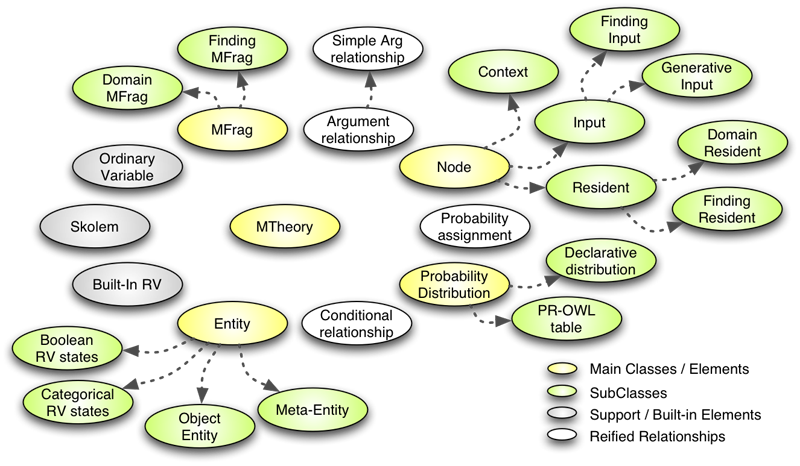
\includegraphics[height=5cm]{./images/prowl1}
	\caption{PR-OWL 1.0}
	\label{fig:prowl1}
\end{figure}

Em sua primeira versão chamada PR-OWL 1.0, foi criada uma super ontologia mostrada na figura~\ref{fig:prowl1} que fazia uma simulação da estrutura de um MEBN. Aquela super ontologia podia ser usada em Protegé para construir ontologias probabilísticas. Mas como se ve na figura~\ref{fig:protege}, usá-la nessa ferramenta era complexo pela sua estrutura.

Para solucionar aquele problema, no ano 2010, apareceu PR-OWL 2.0, que podia ser usada só na ferramenta UnBBayes~\cite{UnBBayes08} (Figura~\ref{fig:unbbayes}, desenvolvida exclusivamente para construir ontologias probabilísticas do mesmo jeito que Protegé fazia com as ontologias comuns. Apesar disso, UnBBayes permite exportar arquivos .owl que são compatíveis para ser usados em Protegé, mas que tem a estrutura da super ontologia anteriormente mencionada.

\begin{figure}[h]
	\centering
	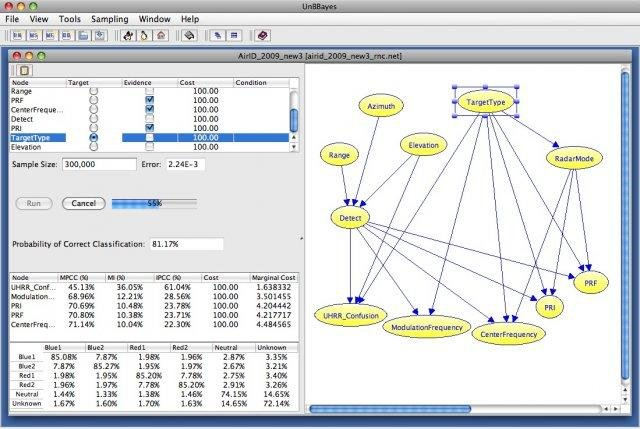
\includegraphics[height=7cm]{./images/unbbayes}
	\caption{Interface gráfica de UnBBayes}
	\label{fig:unbbayes}
\end{figure}